\documentclass[12pt]{article} % Set the font size to 12pt
\usepackage[margin=2.5cm]{geometry} % Set the margin 

% Packages
\usepackage{amsmath} % For mathematical symbols and equations
\usepackage{graphicx} % For including images
\usepackage{lipsum} % For generating dummy text
\usepackage{mathtools} % For mathematical symbols and equations
\usepackage{amssymb} % For mathematical symbols and equations
\usepackage{hyperref} % For hyperlinks
\usepackage{natbib} % For bibliography
% Document information
\title{Resource Reallocation with Carbon Emission Policies}
\author{Seyyed Morteza Aghajanzadeh}
\date{\today}

\begin{document}

\maketitle

\begin{abstract}
    Governments worldwide are implementing policies to mitigate carbon emissions, necessitating significant economic resource reallocation. This study investigates the economic consequences of these shifts, focusing on quantifying reallocation costs and delineating conditions for optimal resource distribution. Utilizing a model of a closed economy characterized by monopolistic competition and firm heterogeneity, the study distinguishes between 'green' (eco-friendly) and 'brown' (fossil fuel-dependent) capital in the production function. The emission function has been extended to incorporate variable parameters that reflect the environmental impacts of these resources. This analysis aims to provide critical insights into the dynamics of resource allocation under environmental policy constraints, underscoring the trade-offs between economic output and environmental sustainability. The results are intended to guide policymaking by clarifying the economic costs associated with transitioning to a low-carbon economy and outlining strategies to balance environmental and economic objectives optimally.    
\end{abstract}

\section*{Environment and Technology}

\begin{itemize}
    \item Total real output is:
    \begin{equation}
    Y = \Pi_1^S Y_s^{\lambda_s}, \quad \text{where} \quad \sum^S \lambda_s = 1
\end{equation}

    \item The real output in each sector $s$ is:
    \begin{equation}
    Y_s = \left(
        \sum_{i=1}^I Y_{si}^{\frac{\sigma_s-1}{\sigma_s}}
    \right)^{\frac{\sigma_s}{\sigma_s-1}}
\end{equation}

    \item The real output for firms $i$ in sector $s$ is:
	\begin{equation}
    \label{eq:firm_output}
    Y_{si} = \hat{A}_{si}\hat{K}_{si}^{\beta_s} L_{si}^{1-\beta_s}
    \quad,\qquad\hat{K} = (
        \alpha_s G_{si}^{\frac{\gamma_s-1}{\gamma_s}} + (1-\alpha_s) B_{si}^{\frac{\gamma_s-1}{\gamma_s}}
    ) ^ {\frac{\gamma_s}{\gamma_s-1}}
\end{equation}
    
	\item The firm's emission is:
	\begin{equation}
    \label{eq:firm_emission}
    E_{si} = \tilde{A}_{si}\tilde{K}_{si}^{\theta_s} L_{si}^{1-\theta_s} \quad,\qquad \tilde{K} = (
        \mu_s G_{si}^{\frac{\eta_s-1}{\eta_s}} + (1-\mu_s) B_{si}^{\frac{\eta_s-1}{\eta_s}}
    ) ^ {\frac{\eta_s}{\eta_s-1}}
\end{equation}

    \item The nominal profit for firms:
    \begin{equation}
    \pi_{si} = (1+\tau_{s}^p) P_{s} Y_{s} - \left(\left[
        (1+ \tau_{G_{s}}) r_{si}G_{si} + (1+ \tau_{B_{s}}) r_{si}B_{si} + (1+ \tau_{l_{s}}) w_{si}l_{si}
    \right] + {\tau_{E} E_{si}}\right)
\end{equation}
    
\end{itemize}
\section*{Optimal Allocation}
\begin{itemize}
    \item To maximize profit, the firm follows a two-step process. First, it determines the optimal combination of capital and labor. Then, it selects the appropriate price level.
    \begin{equation*}
    \begin{split}
        \min_{GK_{si}, BK_{si}} & \quad
        \left[
        (1+ \tau_{G_{s}}) r_{si}G_{si} + (1+ \tau_{B_{s}}) r_{si}B_{si} + (1+ \tau_{l_{s}}) w_{si}l_{si}
    \right] + {\tau_{E} E_{si}} \\
        \text{s.t.} & \quad \hat{A}_{si}\hat{K}_{si}^{\beta_s} L_{si}^{1-\beta_s} = \bar{Y}_{si}\\
        % & \quad \tilde{A}_{si}\tilde{K}_{si}^{\theta_s} L_{si}^{1-\theta_s} = E_{si}
    \end{split}
\end{equation*}

    \begin{equation*}
    \max  \quad
     - 		Cost \quad \text{s.t.} \quad \quad \hat{A}_{si}\hat{K}_{si}^{\beta_s} L_{si}^{1-\beta_s} = \bar{Y}_{si}
\end{equation*}
\begin{equation*}
z^k_{si} \equiv \frac{G_{si}}{B_{si}} = \left[
    \frac{\alpha_s}{1-\alpha_s} \dfrac{\frac{\partial }{\partial B}Cost_{si}}{\frac{\partial }{\partial G}Cost_{si}}
\right] ^ {\gamma_s} 
\end{equation*}
then we can rewrite the optimal capital level as:
\begin{equation*}
    \begin{split}
        \hat{K}_{si} &= B_{si}(\alpha_s {z^k_{si}}^{\frac{\gamma_s -1}{\gamma_s}} + (1-\alpha_s))^{\frac{\gamma_s}{\gamma_s - 1}}\\
        & = G_{si}(\alpha_s  + (1-\alpha_s){z^k_{si}}^{(1-\gamma_s )})^{\frac{\gamma_s}{\gamma_s - 1}}
    \end{split}
\end{equation*}
and then the optimal labor ratio is:
\begin{equation*}
    \begin{split}
    z^l_{si} \equiv \frac{L_{si}}{\hat{K}_{si}} & = \frac{1-\beta_s}{\beta_s} \frac{1}{1-\alpha_s} (\alpha_s {z^k_{si}}^{(\gamma_s -1)} + (1-\alpha_s))^{\frac{1}{1-\gamma_s}}\dfrac{\frac{\partial }{\partial B}Cost_{si}}{\frac{\partial }{\partial L}Cost_{si}}\\
    & = \frac{1-\beta_s}{\beta_s} \frac{1}{\alpha_s}(\alpha_s  + (1-\alpha_s){z^k_{si}}^{(1-\gamma_s )})^{\frac{1}{1-\gamma_s}}\dfrac{\frac{\partial }{\partial G}Cost_{si}}{\frac{\partial }{\partial L}Cost_{si}}
\end{split}
\end{equation*}

    \item Let's define the use the optimal ratios ($z^k_{si} \equiv (\frac{G_{si}}{B_{si}})*$ and $z^l_{si} \equiv (\frac{L_{si}}{\hat{K}_{si}})^*$)
    
    \item Optimal capital level for given output is (see appendix \ref{Ap:optimal level for given output} for proof):
    \begin{equation*}
    G_{si}^* = \frac{\bar{Y}_{si}}{\hat{A}_{si}} \left(
        \alpha_s  + (1-\alpha_s){z^k_{si}}^{(1-\gamma_s )}
    \right)^{\frac{\gamma_s}{1-\gamma_s}} {z_{si}^l}^{(1-\beta_s)}
\end{equation*}
\begin{equation*}
    B_{si}^* = \frac{\bar{Y}_{si}}{\hat{A}_{si}} \left(\alpha_s {z^k_{si}}^{\frac{\gamma_s -1}{\gamma_s}} + (1-\alpha_s)
    \right)^{\frac{\gamma_s}{1-\gamma_s}} {z_{si}^l}^{(\beta_s-1)}
\end{equation*}
\begin{equation*}
    L_{si}^* = \frac{\bar{Y}_{si}}{\hat{A}_{si}}  {z_{si}^l}^{-\beta_s}
\end{equation*}

    \item The emission level for given output is (see appendix \ref{Ap:emission optimal level} for proof):
    \begin{equation}
    E_{si} = {\frac{\tilde{A}_{si}}{\hat{A}_{si}}(\frac{\phi_{si}}{z^{l}_{si}})^{\theta_s} {z^{l}_{si}}^{\beta_s}} \bar{Y}_{si} = \psi_{si}\bar{Y}_{si}, \quad \text{where} \quad \phi_{si}  = \frac{(\mu_s  + (1-\mu_s){z^k_{si}}^{(1-\eta_s )})^ {\frac{\eta_s}{\eta_s-1}}}{(\alpha_s  + (1-\alpha_s){z^k_{si}}^{(1-\gamma_s )}) ^{\frac{\gamma_s}{\gamma_s-1}}} 
\end{equation}
    
    \item The cost of production is (see appendix \ref{Ap:cost minimization function} for details of the definition):
    \begin{equation*}
    \begin{split}
        \Rightarrow C(\bar{F}_{si}) &  = \left[
            (1+ \tau_{G_{si}}) r^{G}_{si}G_{si} + (1+ \tau_{B_{si}}) r^{K}_{si}B_{si} + (1+ \tau_{l_{si}}) w_{si}l_{si}
        \right] + {\tau_{E} E_{si}} \\
        & = C_{si} \bar{F}_{si}  \\
    \end{split}
\end{equation*}
    
    \item The optimal price level is (see appendix \ref{Ap:firm_price} for proof):
    \begin{equation}
    \begin{split}
         P_{si} =& \frac{1}{1+\tau_{si}^p}\frac{\sigma_s}{\sigma_s - 1} C_{si} \\
    \end{split}
\end{equation}

\end{itemize}

\section*{Calibration}
I need to calibrate the model to match the summary statistics of the \cite{martinsson2024effect}. In order to be able to use the table in the paper, I need to make some simplifying assumptions. First, I assume that $\sigma = \infty$ to simplify the ratios to $E/PY$. Second, I assume that $\mu_s = 0$ and $\theta_s = 1$ to simplify the emission function ($
    E_{si} = \tilde{A}_{si}B_{si}
$). Third, I assume that there is no friction in the market, so $\tau_{si}^p = \tau_{G_{si}} = \tau_{B_{si}} = \tau_{l_{si}} = 0$ to simplify the profit function.
Now the profit is:
    \begin{equation*}
        \begin{split}
            \pi_{si} &=  P_{si} Y_{si} - (        r^{G}_{si}G_{si} + r^{B}_{si}B_{si} + w_{si}l_{si} + {\tau_{E} E_{si}})\\
            & = P_{si} Y_{si} - (r_{{si}}^GG_{si}  + (r_{{si}}^B + \tau_E\tilde{A}_{si})B_{si} +  w_{si}l_{si})
        \end{split}
    \end{equation*}
    and the simplified economy is:

    \input{model_elements/simplified model}

Based on the information provided in Table 2 of the paper by \cite{martinsson2024effect}, I can set the value of $\beta$ to 0.6 in order to match the capital intensity. Additionally, I can set the values of $r_B$ and $r_G$ to 11\% to match the return on capital. To match the number of firms in the sector, I can set the number of firms to $1200$. Furthermore, I can set the mean and standard deviation of labor to $250$ and $900$, respectively, to match the labor distribution. Finally, I can set the wage to $500,000$ SEK to match the wage in Sweden. In order to match the summary statistics of the emission-to-sales ratio (approximately $0.0072$), the elasticity of carbon tax on emissions' intensity (approximately $2$), and the total output in the economy (approximately $10$ BSEK), I need to determine appropriate values for $\alpha_s$, $\gamma_s$, $\hat{A}$, and $\tilde{A}$.

Here is the sensetivity of the model to the $\alpha_s$ and $\gamma_s$:
    \begin{figure}[http]
		\centering
		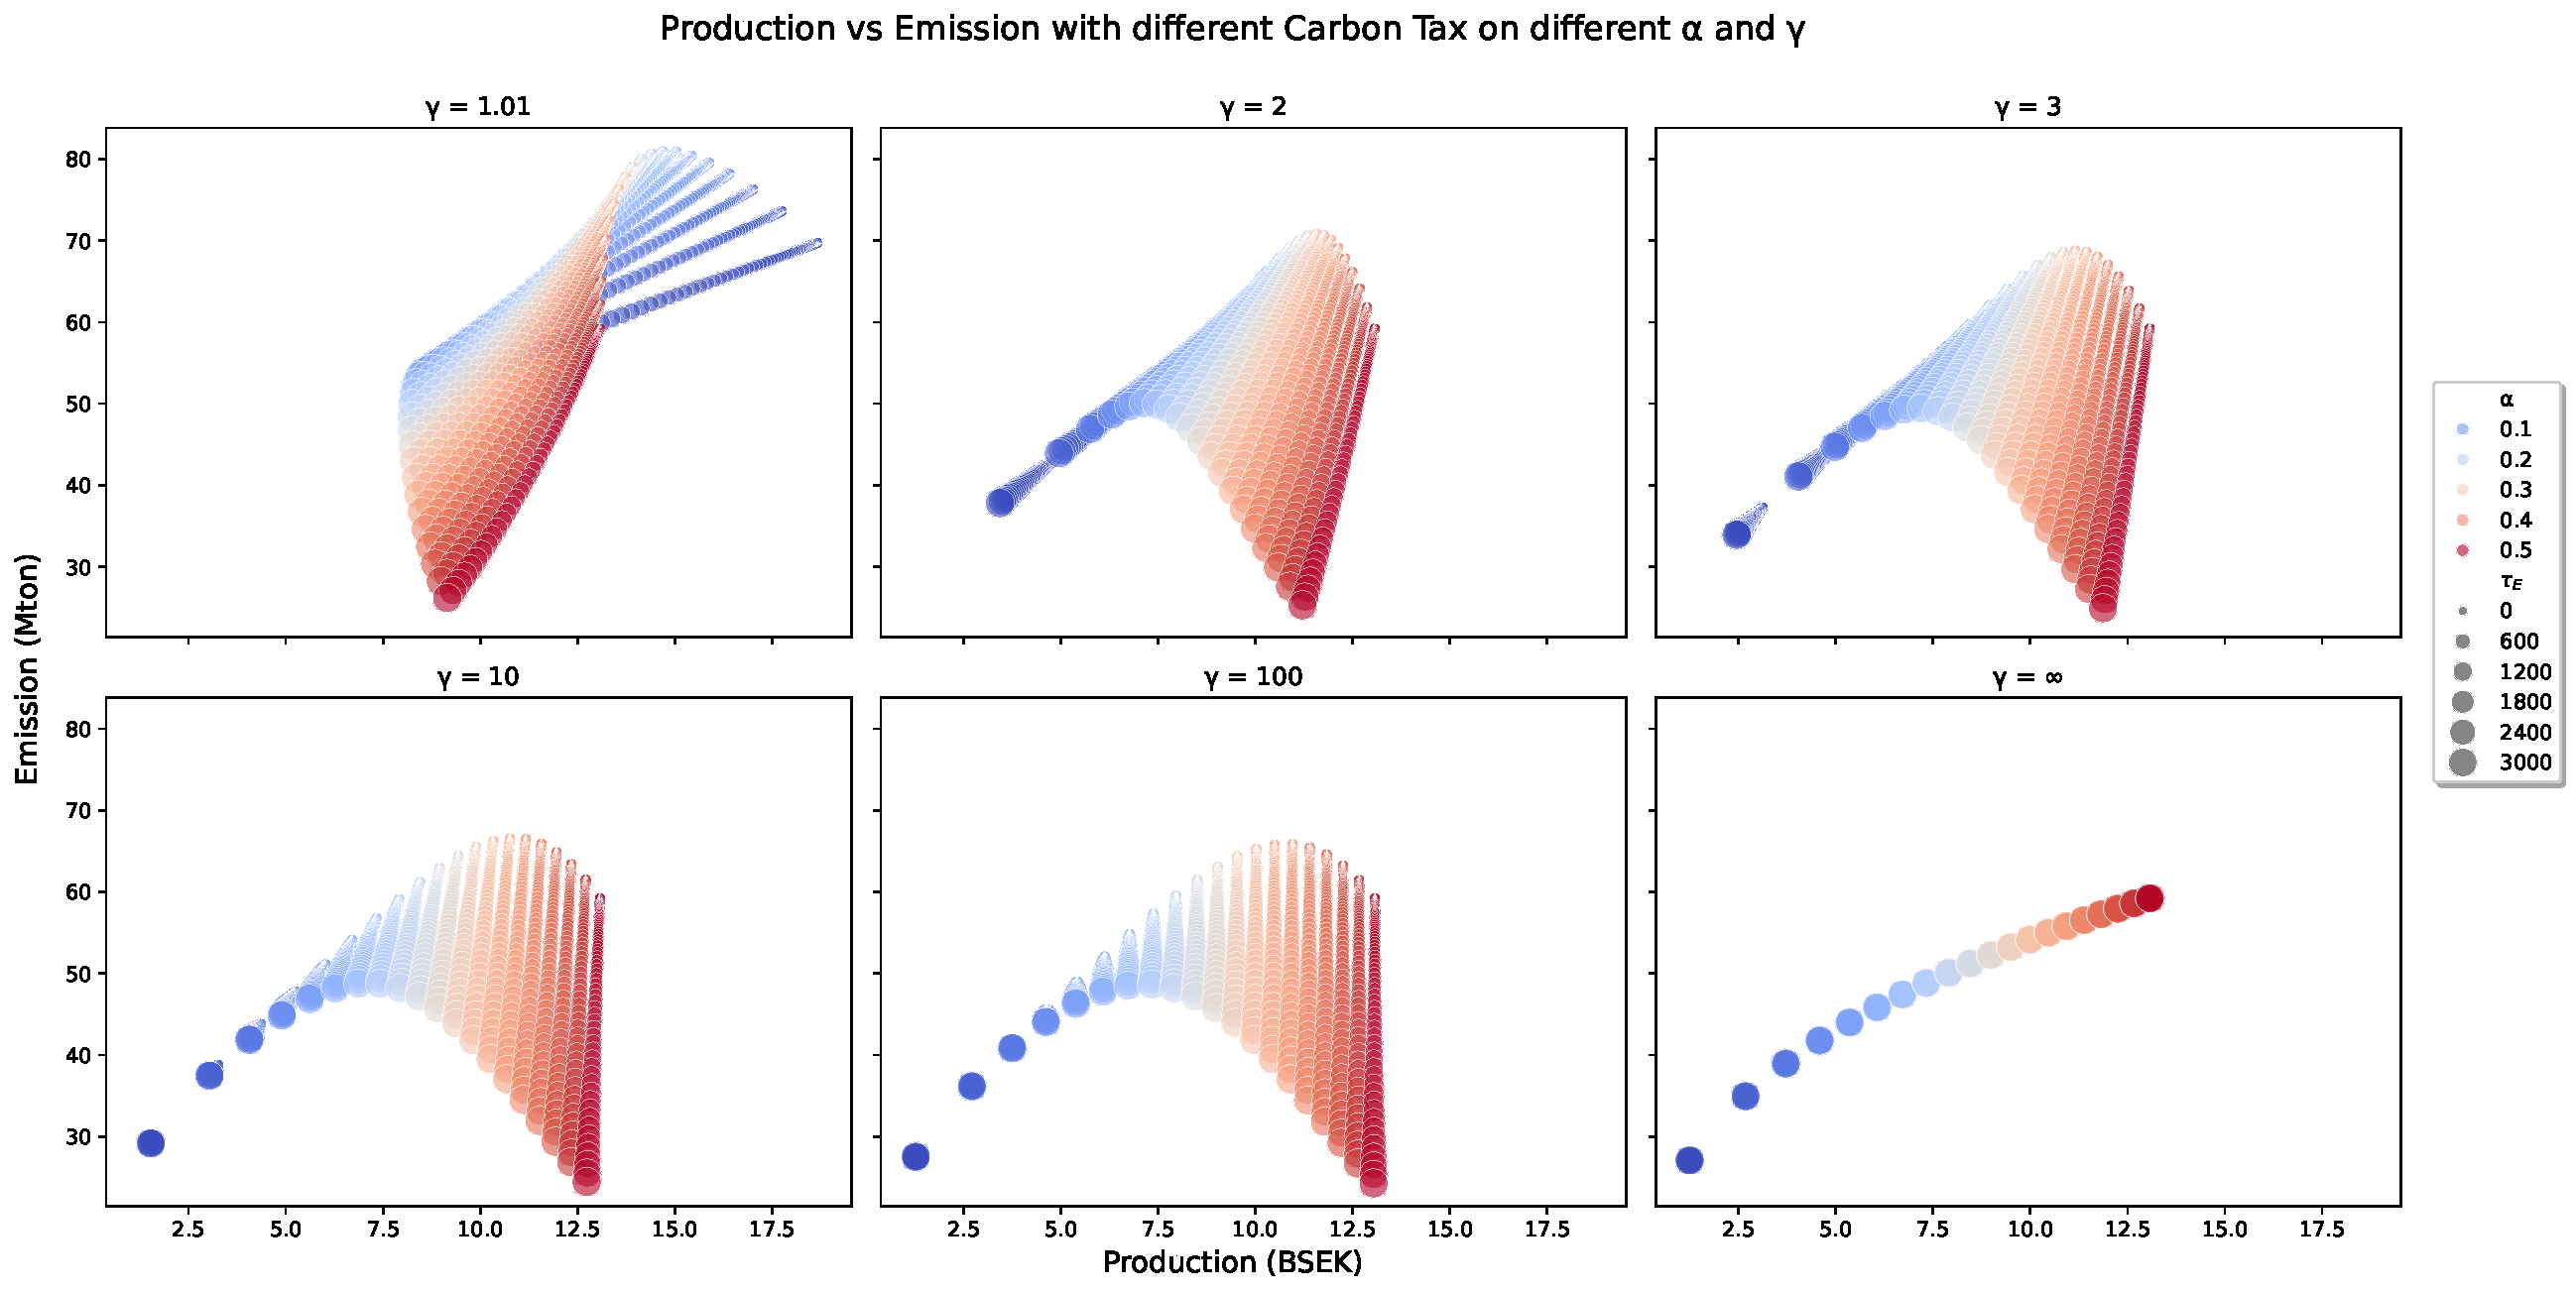
\includegraphics[width=0.9\textwidth]{Figures/production_emission.pdf}
	\end{figure}

I need to determine the values of $\alpha_s$ and $\gamma_s$ to match the elasticity of carbon tax on emissions' intensity and the emission-to-sales ratio. To do this, I can simulate the model for different values of $\alpha_s$ and $\gamma_s$ and calculate the resulting elasticity of carbon tax on emissions' intensity and the emission-to-sales ratio. Based on my simulations, I have found that in order to match the emission-to-sales ratio and the total output of approximately 10 BSEK in the economy, I need to set the average values of $\hat{A}$ to \input{values/A hat estimate} and $\tilde{A}$ to \input{values/A tilde estimate}. Additionally, to match the elasticity of carbon tax on emissions' intensity, I need to set $\alpha_s$ to \input{values/alpha estimate} and $\gamma_s$ to \input{values/gamma estimate}.
    


One insightful approach is to evaluate three distinct environmental policies: a carbon tax, a green subsidy, and a brown tax. The green subsidy is implemented as a reduction in the interest rate on green capital, ranging from $0\%$ to $100\%$. Conversely, the brown tax is applied as an additional charge on the interest rate for brown capital, varying from $0\%$ to $400\%$. 

Using the calibrated model, I simulate the impact of these policies on the carbon intensity of the economy. The outcomes are illustrated in following figure, which displays the effects of each policy on reducing carbon intensity. It is evident from the results that the carbon tax is the most effective policy for lowering carbon intensity. Specifically, a carbon tax of $100$ SEK per unit of emissions is roughly equivalent in impact to a \input{values/100 SEK tax equivalent} discount on the interest rate for green capital, underscoring the significant potential of fiscal measures in promoting environmental sustainability. Brown tax cannot achieve the same level of reduction in carbon intensity as the carbon tax, highlighting the importance of targeted policy interventions in addressing environmental challenges.


\begin{figure}[http]
    \centering
    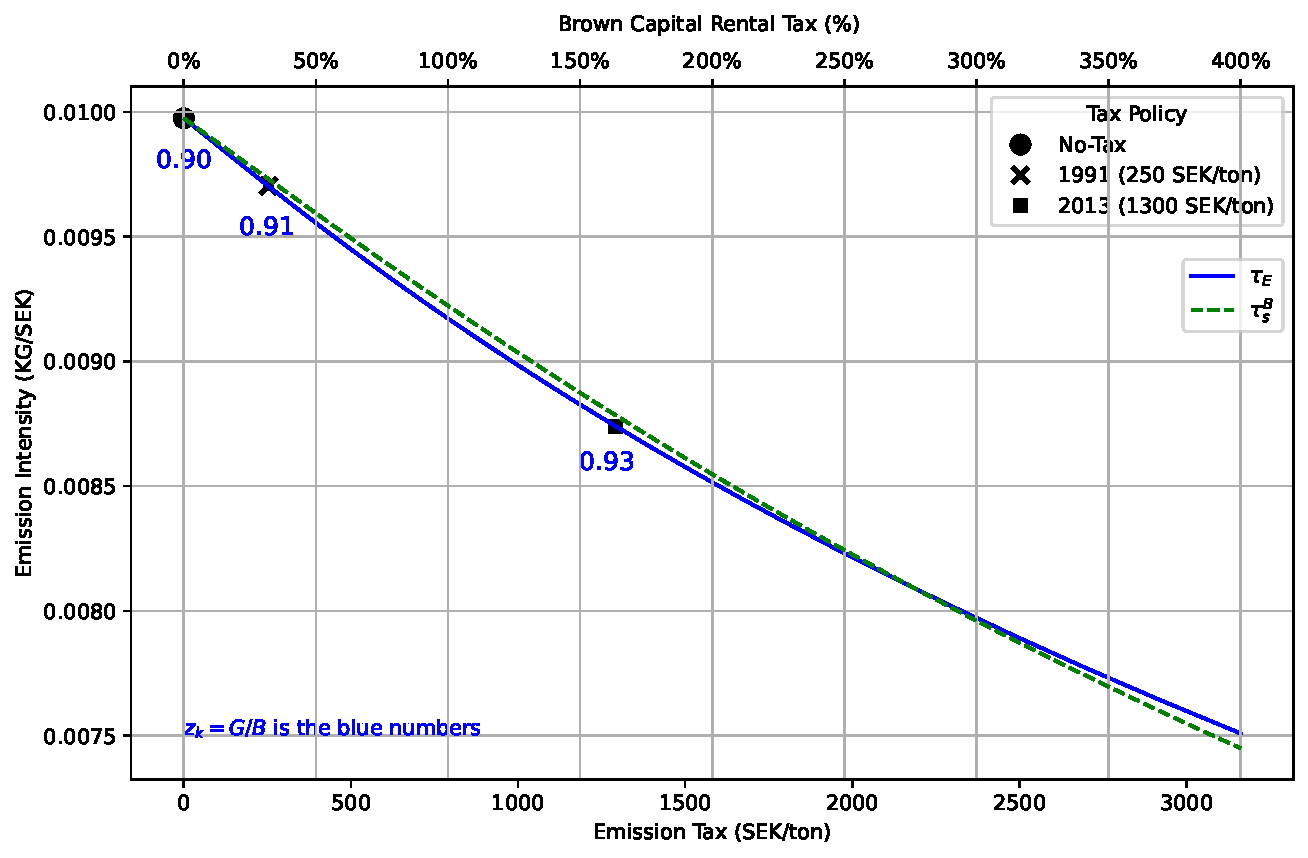
\includegraphics[width=.8\textwidth]{Figures/intensity_tax_premium.pdf}
\end{figure}



\section*{Technology}
We need to find an expression for the technologies ($\hat{A}_{si}$ and $\tilde{A}_{si}$) based on observable variables. (see appendix \ref{Ap:Productiontechnology} and \ref{Ap:Emissiontechnology} for proof)

\begin{equation*}
    \hat{A}_{si} = \nu_s \dfrac{(P_{si}Y_{si})^{\frac{\sigma_s}{\sigma_s-1}}}{\hat{K}_{si}^{\beta_s} L_{si}^{1-\beta_s}}, \quad \text{where} \quad \nu_s = \frac{1}{P_s(P_sY_s)^{\frac{1}{\sigma_s-1}}}
\end{equation*}

\begin{equation*}
    \tilde{A}_{si} = \dfrac{E_{si}}{\tilde{K}_{si}^{\theta_s} L_{si}^{1-\theta_s}}
\end{equation*}



\section*{Reallocation}
Given the optimal ratios of the firm, the allocation of resources is (see appendix \ref{Ap:reallocation} for proof):
\begin{gather*}\label{eq:allocation_social_planner_L}
    \hat{L}_{si} = \dfrac{\hat{A}_{si}^{\sigma -1}}{\sum_j \hat{A}_{sj}^{\sigma -1}}L_s\\ 
    \tilde{L}_{si} = \dfrac{\hat{A}_{si}^{\sigma -1}/\tilde{A}_{si}^{\sigma}}{\sum_j \hat{A}_{sj}^{\sigma -1}/ \tilde{A}_{sj}^{\sigma}}L_s
\end{gather*}
\begin{gather*}
    B_s = \dfrac{1}{1 + z_s^k} K_s \\ 
    G_s = \dfrac{z_s^k}{1 + z_s^k} K_s
\end{gather*}
\begin{gather*}\label{eq:allocation_social_planner_G}
    \hat{G}_{si} = \dfrac{\hat{A}_{si}^{\sigma -1}}{\sum_j \hat{A}_{sj}^{\sigma -1}}G_s\\ 
    \tilde{G}_{si} = \dfrac{\hat{A}_{si}^{\sigma -1}/\tilde{A}_{si}^{\sigma}}{\sum_j \hat{A}_{sj}^{\sigma -1}/ \tilde{A}_{sj}^{\sigma}}G_s
\end{gather*}
\begin{gather*} \label{eq:allocation_social_planner_B}
    \hat{B}_{si} = \dfrac{\hat{A}_{si}^{\sigma -1}}{\sum_j \hat{A}_{sj}^{\sigma -1}}B_s\\ 
    \tilde{B}_{si} = \dfrac{\hat{A}_{si}^{\sigma -1}/\tilde{A}_{si}^{\sigma}}{\sum_j \hat{A}_{sj}^{\sigma -1}/ \tilde{A}_{sj}^{\sigma}}B_s
\end{gather*}

Once the optimal allocation of resources is determined, it becomes possible to calculate the optimal real output and emission levels for individual firms, sectors, and the overall economy.

Following, by substituting the observed levels into the production function and emission function, the actual real output and emission values can be obtained for each firm, sector, and the economy as a whole.

Once I know the optimal allocation of resources, I can determine the optimal real output and emission for a firm, a sector, and the economy. 
Given the optimal levels, I can replace the optimal levels in the production function and emission function with the actual observed levels to determine the real output and emission for each firm, sector, and the economy.


\section*{Wedges}
\begin{itemize}
    \item The marginal nominal product of each input should be equal to the marginal cost of that for the maximizing firm (see appendix \ref{Ap:wedges} for proof).
	\begin{gather*}
    \alpha_s \beta_s  \frac{\sigma_s-1}{\sigma_s} \frac{P_{si}Y_{si}}{\hat{K}_{si}}(\frac{\hat{K}_{si}}{G_{si}})^{\frac{1}{\gamma_s}} = \frac{\partial Cost_{si}}{\partial G_{si}} \\\\
    (1-\alpha_s) \beta_s  \frac{\sigma_s-1}{\sigma_s} \frac{P_{si}Y_{si}}{\hat{K}_{si}}(\frac{\hat{K}_{si}}{B_{si}})^{\frac{1}{\gamma_s}} = \frac{\partial Cost_{si} }{\partial B_{si}}\\\\
    (1-\beta_s) \frac{\sigma_s-1}{\sigma_s} \frac{P_{si}Y_{si}}{L_{si}} = \frac{\partial Cost_{si}}{\partial L_{si}} \\\\
\end{gather*}
\end{itemize}


\section*{Estimation}
I will follow the \cite{kmenta1967estimation} to estimate the parameters of the model. The production function is:
\begin{gather*}
    Y_{it} = \hat{A}_{it}(
        \alpha G_{it}^{\frac{\gamma-1}{\gamma}} + (1-\alpha) B_{it}^{\frac{\gamma-1}{\gamma}}
    ) ^ {\frac{\beta\gamma}{\gamma-1}} L_{it}^{1-\beta}\\
    \ln Y_{it} = \ln \hat{A}_{it} + \frac{\beta\gamma}{\gamma-1} \ln(
        \alpha G_{it}^{\frac{\gamma-1}{\gamma}} + (1-\alpha) B_{it}^{\frac{\gamma-1}{\gamma}}
    ) + (1-\beta) \ln L_{it}
\end{gather*}
I assume that the $\hat{A}_{it} \equiv e^a e^{u_{it}}$, where $a$ is the common component of productivity and $u_{it}$ is the unpredictable component. We can rewrite the production function as:
\begin{gather*}
    \ln Y_{it} = a + u_{it} + \frac{\beta\gamma}{\gamma-1} \ln(
        \alpha G_{it}^{\frac{\gamma-1}{\gamma}} + (1-\alpha) B_{it}^{\frac{\gamma-1}{\gamma}}
    ) + (1-\beta) \ln L_{it}
\end{gather*}
Following the \cite{kmenta1967estimation}, I take the first-order approximation of the production function around the $\gamma_s = 1$. This requires to take the limit of the third term in the production function as $\gamma_s$ approaches 1. The limit is:
\begin{gather*}
    \lim_{\gamma_s \to 1} \frac{\beta\gamma}{\gamma-1} \ln(
        \alpha G_{it}^{\frac{\gamma-1}{\gamma}} + (1-\alpha) B_{it}^{\frac{\gamma-1}{\gamma}}
    ) = \beta (\alpha \ln G_{it}   + (1-\alpha)\ln B_{it} )
\end{gather*}
and the limit of the derivative of this same term
\begin{gather*}
    \lim_{\gamma_s \to 1} \frac{\partial}{\partial \gamma_s} \left( \frac{\beta\gamma}{\gamma-1} \ln(
        \alpha G_{it}^{\frac{\gamma-1}{\gamma}} + (1-\alpha) B_{it}^{\frac{\gamma-1}{\gamma}}
    ) \right) = \beta \frac{\alpha (1-\alpha)}{2}(\ln G_{it} - \ln B_{it})^2
\end{gather*}
The first-order approximation of the production function is:
\begin{gather*}
    \ln Y_{it} = a + u_{it} +  \beta\alpha \ln G_{it}   + \beta(1-\alpha)\ln B_{it} + (1-\beta) \ln L_{it} + \beta \frac{\alpha (1-\alpha)(\gamma_s - 1)}{2}(\ln G_{it} - \ln B_{it})^2
\end{gather*}

To estimate this approximation, we can use OLS with firm fixed effects and appropriately defined coefficients:
\begin{gather*}
    \ln Y_{it} = \beta_0^Y + \beta_G^Y \ln G_{it} + \beta_B^Y \ln B_{it} + \beta_L^Y \ln L_{it} + \beta_{GB}^Y (\ln G_{it} - \ln B_{it})^2 + \epsilon_{it}
\end{gather*}
then we can derive the parameters of the model as:
\begin{table}[http]
    \centering
    \begin{tabular}{cc}
        \hline
        \textbf{Parameter} & \textbf{Value} \\
        \hline
        $\beta_{s}$ & $1-\beta_L^Y$ \vspace{5pt}
        \\
        $\alpha_{s}$ & $1-\dfrac{\beta_B^Y}{1-\beta_L^Y}$ \vspace{5pt}
        \\
        $\gamma_{s}$ & $1+\dfrac{2\beta_{GB}^Y(1-\beta_L^Y)}{\beta_G^Y\beta_B^Y}$ \vspace{5pt}
        \\
        \hline
    \end{tabular}
\end{table}

I can use the same approach to estimate the emission function. The estimation model is:
\begin{gather*}
    \ln E_{it} = \beta_0^E + \beta_G^E \ln G_{it} + \beta_B^E \ln B_{it} + \beta_L^E \ln L_{it} + \beta_{GB}^E (\ln G_{it} - \ln B_{it})^2 + \epsilon_{it}
\end{gather*}
and the parameters of the emission function are:
\begin{table}[http]
    \centering
    \begin{tabular}{cc}
        \hline
        \textbf{Parameter} & \textbf{Value} \\
        \hline
        $\theta_{s}$ & $1-\beta_L^E$ \vspace{5pt}
        \\
        $\mu_{s}$ & $1-\dfrac{\beta_B^E}{1-\beta_L^E}$ \vspace{5pt}
        \\
        $\eta_{s}$ & $1+\dfrac{2\beta_{GB}^E(1-\beta_L^E)}{\beta_G^E\beta_B^E}$ \vspace{5pt}
        \\
        \hline
    \end{tabular}
\end{table}






\newpage

\appendix
\section{Definitions and Proofs} 
\subsection{Optimal level for given output} \label{Ap:optimal level for given output}
\begin{equation*}
    \bar{Y}_{si} = \hat{A}_{si} \hat{K^*}_{si}^{\beta_s} {L^*}_{si}^{1-\beta_s} = \hat{A}_{si} \hat{K^*}_{si} ({\frac{L^*}{\hat{K^*}}})_{si}^{(1-\beta_s)}= \hat{A}_{si} \hat{K^*}_{si} {z_{si}^l}^{(1-\beta_s)}
\end{equation*}
we can rewrite the optimal capital level as:
\begin{equation*}
    \begin{split}
        \hat{K}_{si} &= B_{si}(\alpha_s {z^k_{si}}^{\frac{\gamma_s -1}{\gamma_s}} + (1-\alpha_s))^{\frac{\gamma_s}{\gamma_s - 1}}\\
        & = G_{si}(\alpha_s  + (1-\alpha_s){z^k_{si}}^{(1-\gamma_s )})^{\frac{\gamma_s}{\gamma_s - 1}}
    \end{split}
\end{equation*}
and then drive the optimal level of each type of capital:
\begin{equation*}
    G_{si}^* = \frac{\bar{Y}_{si}}{\hat{A}_{si}} \left(
        \alpha_s  + (1-\alpha_s){z^k_{si}}^{(1-\gamma_s )}
    \right)^{\frac{\gamma_s}{1-\gamma_s}} {z_{si}^l}^{(1-\beta_s)}
\end{equation*}
\begin{equation*}
    B_{si}^* = \frac{\bar{Y}_{si}}{\hat{A}_{si}} \left(\alpha_s {z^k_{si}}^{\frac{\gamma_s -1}{\gamma_s}} + (1-\alpha_s)
    \right)^{\frac{\gamma_s}{1-\gamma_s}} {z_{si}^l}^{(\beta_s-1)}
\end{equation*}
\begin{equation*}
    L_{si}^* = \frac{\bar{Y}_{si}}{\hat{A}_{si}}  {z_{si}^l}^{-\beta_s}
\end{equation*}

\subsection{Emission optimal level} \label{Ap:emission optimal level}
First we need to convert the production capital ($\hat{K}_{si}$) to the emission capital ($\tilde{K}_{si}$):
\begin{equation*}
    \begin{split}
        \tilde{K} = (
        \mu_s G_{si}^{\frac{\eta_s-1}{\eta_s}} + (1-\mu_s) B_{si}^{\frac{\eta_s-1}{\eta_s}}
    ) ^ {\frac{\eta_s}{\eta_s-1}} = G_{si}(\mu_s  + (1-\mu_s){z^k_{si}}^{(1-\eta_s )})^ {\frac{\eta_s}{\eta_s-1}}\\
    \hat{K} = (
        \alpha_s G_{si}^{\frac{\gamma_s-1}{\gamma_s}} + (1-\alpha_s) B_{si}^{\frac{\gamma_s-1}{\gamma_s}}
    ) ^ {\frac{\gamma_s}{\gamma_s-1}} = G_{si}(\alpha_s  + (1-\alpha_s){z^k_{si}}^{(1-\gamma_s )})^ {\frac{\gamma_s}{\gamma_s-1}}
    \end{split}
\end{equation*}
\begin{equation*}
    \Rightarrow \phi_{si} \equiv \frac{\tilde{K}}{\hat{K}} = \frac{(\mu_s  + (1-\mu_s){z^k_{si}}^{(1-\eta_s )})^ {\frac{\eta_s}{\eta_s-1}}}{(\alpha_s  + (1-\alpha_s){z^k_{si}}^{(1-\gamma_s )}) ^{\frac{\gamma_s}{\gamma_s-1}}} = \frac{(\mu_s {z^k_{si}}^{(\eta_s -1)}  + (1-\mu_s))^ {\frac{\eta_s}{\eta_s-1}}}{(\alpha_s {z^k_{si}}^{(\gamma_s -1)}  + (1-\alpha_s))^{\frac{\gamma_s}{\gamma_s-1}}}
\end{equation*}
As we can see the $\phi_{si}$ is a function of $z^k_{si}$, $\mu_s$, $\alpha_s$ and $\gamma_s$. Now we can calculate the optimal emission level ($E_{si}$) as follows:
\begin{equation*}
    \begin{split}
        E_{si} &= \tilde{A}_{si}\tilde{K}_{si}^{\theta_s} L_{si}^{1-\theta_s} = \tilde{A}_{si} \tilde{K}_{si} ({\frac{L_{si}}{\tilde{K}_{si}}})^{1-\theta_s}\\
    &= \tilde{A}_{si} (\phi_{si} \hat{K}_{si}) ({\frac{L_{si}}{\phi_{si} \hat{K}_{si}}})^{1-\theta_s}\\
    &= {\tilde{A}_{si}}{\phi_{si}}^{\theta_s} \hat{K}_{si} {z^{l}_{si}}^{1-\theta_s} \\
   & = {\tilde{A}_{si}}{\phi_{si}}^{\theta_s}{z^{l}_{si}}^{\beta_s-\theta_s}\hat{K}_{si}{z^{l}_{si}}^{1-\beta_s}\\
   & = \frac{\tilde{A}_{si}}{\hat{A}_{si}}(\frac{\phi_{si}}{z^{l}_{si}})^{\theta_s} {z^{l}_{si}}^{\beta_s} \bar{Y}_{si}
    \end{split}
\end{equation*}


\subsection{Cost Minimization function} \label{Ap:cost minimization function}
\begin{equation*}
	C(\bar{F}_{si}) = C_{si} \bar{F}_{si} 
	\end{equation*}
	\begin{equation*}
		\begin{split}
			\text{where} \quad C_{si}  &  = (1+ \tau_{G_{si}}) r^{G}_{si} \frac{1}{\hat{A}_{si}}\left(
				\alpha_s  + (1-\alpha_s){z^k_{si}}^{-\frac{\gamma_s-1}{\gamma_s}}
				\right)^{\frac{\gamma_s}{1-\gamma_s}} {z_{si}^l}^{(\beta_s-1)}\\
			& + (1+ \tau_{B_{si}})r^{B}_{si}\frac{1}{\hat{A}_{si}} \left(\alpha_s {z^k_{si}}^{\frac{\gamma_s -1}{\gamma_s}} + (1-\alpha_s)
			\right)^{\frac{\gamma_s}{1-\gamma_s}} {z_{si}^l}^{(\beta_s-1)}\\
			& + (1+ \tau_{l_{si}}) w_{si} \frac{1}{\hat{A}_{si}}  {z_{si}^l}^{\beta_s}\\
			 & + \tau_{E} \frac{\tilde{A}_{si}}{\hat{A}_{si}}(\frac{\phi_{si}}{z^{l}_{si}})^{\theta_s} {z^{l}_{si}}^{\beta_s}
		\end{split}
	\end{equation*}

\subsection{Sector Price} \label{Ap:sector price}
 We need to solve the sector price $P_s$ as function of firm price $P_{si}$, where $P_s$ is defined as the price of acquiring a unit of the sector benefit:
    \begin{equation*}
    \begin{split}
        \min_{F_{si}} & \quad \left\{
    \sum_{i} P_{si} F_{si}	
    \right\}\\
    \text{s.t.} & \quad \left(\sum_{i} F_{si}^{\frac{\sigma_s-1}{\sigma_s}}\right)^{\frac{\sigma_s}{\sigma_s-1}} = \bar{F}_s
    \end{split}
\end{equation*}
\begin{equation*}
    F.O.C \Rightarrow P_{si}^{\sigma_s} F_{si} = P_s^{\sigma_s} {F}_s
\end{equation*}

\subsection{Firm Price} \label{Ap:firm_price}
We need to solve the firm price $P_{si}$ as function of sector price $P_s$, where $P_{si}$ is defined as the price of acquiring a unit of the firm benefit:
    \begin{gather*}
    \max_{P_{si}} \quad\pi_{si} =  (1+\tau_{si}^p)P_{si}Y_{si} - C_{si} {Y}_{si} \\
    \max  \quad (1+\tau_{si}^p)P_{si}( \frac{P_s}{ P_{si}})^{\sigma_s}{Y}_s - C_{si} (\frac{P_s}{ P_{si}})^{\sigma_s}{Y}_s \\
    \max \quad  (1+\tau_{si}^p)P_{si}^{1-\sigma_s}P_s^{\sigma_s}{Y}_s - C_{si} P_{si}^{-\sigma_s}P_s^{\sigma_s}{Y}_s \\
    \max \quad P_s^{\sigma_s}{Y}_s \left(
        (1+\tau_{si}^p)P_{si}^{1-\sigma_s} - C_{si} P_{si}^{-\sigma_s} 
    \right)\\
    \max \quad  (1+\tau_{si}^p)P_{si}^{1-\sigma_s} - C_{si} P_{si}^{-\sigma_s} \\
    \Rightarrow 0 = P_{si}^{-\sigma_s - 1} \left[
        (1+\tau_{si}^p)(1-\sigma_s)P_{si} + \sigma_s C_{si} 
    \right]
    \\
    \Rightarrow P_{si} = \frac{1}{1+\tau_{si}^p}\frac{\sigma_s}{\sigma_s - 1} C_{si} 
\end{gather*}

\subsection{Production Technology}
\label{Ap:Productiontechnology}
\begin{gather*}
    P_{si}^{\sigma_s} = P_s^{\sigma_s} Y_s Y_{si}^{-1} 
    \Rightarrow (P_{si}Y_{si})^{\sigma_s} = P_s^{\sigma_s} Y_s Y_{si}^{\sigma_s-1}
    \Rightarrow (P_{si}Y_{si})^{\sigma_s} = (P_sY_s)(P_sY_{si})^{\sigma_s-1}\\
    \Rightarrow (P_{si}Y_{si})^{\frac{\sigma_s}{\sigma_s-1}} = (P_sY_s)^{\frac{1}{\sigma_s-1}}P_sY_{si}\\
    \Rightarrow Y_{si} = \dfrac{(P_{si}Y_{si})^{\frac{\sigma_s}{\sigma_s-1}}}{P_s(P_sY_s)^{\frac{1}{\sigma_s-1}}}\\
    \Rightarrow \hat{A}_{si} = \frac{1}{P_s(P_sY_s)^{\frac{1}{\sigma_s-1}}}\dfrac{(P_{si}Y_{si})^{\frac{\sigma_s}{\sigma_s-1}}}{\hat{K}_{si}^{\beta_s} L_{si}^{1-\beta_s}} = \nu_s \dfrac{(P_{si}Y_{si})^{\frac{\sigma_s}{\sigma_s-1}}}{\hat{K}_{si}^{\beta_s} L_{si}^{1-\beta_s}}
\end{gather*}
\subsection{Emission Technology}
\label{Ap:Emissiontechnology}
\begin{gather*}
    E_{si} = \tilde{A}_{si}\tilde{K}_{si}^{\theta_s} L_{si}^{1-\theta_s} \Rightarrow \tilde{A}_{si} = \dfrac{E_{si}}{\tilde{K}_{si}^{\theta_s} L_{si}^{1-\theta_s}}\\
\end{gather*}



\subsection{Reallocation} \label{Ap:reallocation}


It is the social planner's problem to reallocate resources, therefore there is no need to price the inputs. The social planner's problem is to maximize the total real output subject to the resource constraint. Firms in the economy will produce the optimal level of output given the zero cost of inputs. The social planner's problem is:
\input{model_elements/social planner's problem}

Now I will write the lagrangian for the social planner's problem. The social planner's problem is to maximize the total output in the economy subject to the resource constraint. The lagrangian is:
\input{model_elements/social planner's problem - largranian}
where $\lambda_L$, $\lambda_E$ are the lagrange multipliers for the labor and emission constraints, respectively that are normalized by the capital lagrange multiplier. This results in the fact that the relative marginal cost of labor is $\lambda_L$ and the relative marginal cost of acquiring one unit of capital is 1. Now I can use the results from the firm's problem and the optimal input ratios to derive the optimal output and emissions for the social planner. The optimal input ratios are:
\begin{gather}\label{eq:reallocation_firm_input_ratio}
    z_{s}^k = (\frac{\alpha_s}{1-\alpha_s})^{\gamma_s} \\
    z_{s}^l = \frac{1-\beta_s}{\beta_s} \frac{1}{1-\alpha_s} (\alpha_s {z^k_{s}}^{(\gamma_s -1)} + (1-\alpha_s))^{\frac{1}{1-\gamma_s}} \lambda_L
  \end{gather}
Then I can rewrite the optimal output and emissions for firm under the social planner's problem as:
\input{model_elements/social planner's problem - firm output}
and rewrite the lagrangian as:
\begin{gather*}
    \mathcal{L}_s = \left(
        \sum_i \hat{A}_{si} {z_{s}^l}^{-\beta}\hat{L}_{si}^{\frac{\sigma-1}{\sigma}}
    \right)^{\frac{\sigma}{\sigma-1}} + \lambda_L(L_s - \sum_i \hat{L}_{si}) + \lambda_E(E_s - \sum_i \tilde{A}_{si}(\frac{\phi_{s}}{z^{l}_{s}})^{\theta_s} \hat{L}_{si})\\
    \frac{\partial \mathcal{L}_s}{\partial \hat{L}_{si}} = \left(
        \sum_i \hat{A}_{sk} {z_{s}^l}^{-\beta}\hat{L}_{sk}^{\frac{\sigma-1}{\sigma}}
    \right)^{\frac{1}{\sigma-1}}(\hat{A}_{si}{z_{s}^l}^{-\beta})^{\frac{\sigma-1}{\sigma}}\hat{L}_{si}^{-\frac{1}{\sigma}} - \lambda_L - \lambda_E \tilde{A}_{si}(\frac{\phi_{s}}{z^{l}_{s}})^{\theta_s} = 0\\
    \frac{\partial \mathcal{L}_s}{\partial \hat{L}_{sj}} = \left(
        \sum_i \hat{A}_{sk} {z_{s}^l}^{-\beta}\hat{L}_{sk}^{\frac{\sigma-1}{\sigma}}
    \right)^{\frac{1}{\sigma-1}}(\hat{A}_{sj}{z_{s}^l}^{-\beta})^{\frac{\sigma-1}{\sigma}}\hat{L}_{sj}^{-\frac{1}{\sigma}} - \lambda_L - \lambda_E \tilde{A}_{sj}(\frac{\phi_{s}}{z^{l}_{s}})^{\theta_s} = 0
\end{gather*}

There are two possible cases for the optimal allocation of resources. In the first case, the social planner only cares about maximizing total output and does not consider emissions, resulting in $\lambda_E = 0$. In this scenario, the social planner will allocate all available resources to the firm with the highest productivity:
\begin{gather*}
    \lambda_L = \left(
        \sum_i \hat{A}_{sk} {z_{s}^l}^{-\beta}\hat{L}_{sk}^{\frac{\sigma-1}{\sigma}}
    \right)^{\frac{1}{\sigma-1}}(\hat{A}_{si}{z_{s}^l}^{-\beta})^{\frac{\sigma-1}{\sigma}}\hat{L}_{si}^{-\frac{1}{\sigma}} = \left(
        \sum_i \hat{A}_{sk} {z_{s}^l}^{-\beta}\hat{L}_{sk}^{\frac{\sigma-1}{\sigma}}
    \right)^{\frac{1}{\sigma-1}}(\hat{A}_{sj}{z_{s}^l}^{-\beta})^{\frac{\sigma-1}{\sigma}}\hat{L}_{sj}^{-\frac{1}{\sigma}}\\
    \Rightarrow (\frac{\hat{A}_{si}^{\sigma-1}}{\hat{L}_{si}})^{\frac{1}{\sigma}} = (\frac{\hat{A}_{sj}^{\sigma-1}}{\hat{L}_{sj}})^{\frac{1}{\sigma}} \Rightarrow \frac{\hat{L}_{si}}{\hat{L}_{sj}} = \left(
        \frac{\hat{A}_{si}}{\hat{A}_{sj}}
    \right)^{\sigma-1}
\end{gather*}
 
In the second case, the social planner cares about the emissions, and the social planner will allocate all available resources to the firm with the lowest emissions:
\begin{gather*}
    \lambda_E = \dfrac{\left(
        \sum_i \hat{A}_{sk} {z_{s}^l}^{-\beta}\hat{L}_{sk}^{\frac{\sigma-1}{\sigma}}
    \right)^{\frac{1}{\sigma-1}}(\hat{A}_{si}{z_{s}^l}^{-\beta})^{\frac{\sigma-1}{\sigma}}\hat{L}_{si}^{-\frac{1}{\sigma}}}{
        \tilde{A}_{si}(\frac{\phi_{s}}{z^{l}_{s}})^{\theta_s}
    } = \dfrac{\left(
        \sum_i \hat{A}_{sk} {z_{s}^l}^{-\beta}\hat{L}_{sk}^{\frac{\sigma-1}{\sigma}}
    \right)^{\frac{1}{\sigma-1}}(\hat{A}_{sj}{z_{s}^l}^{-\beta})^{\frac{\sigma-1}{\sigma}}\hat{L}_{sj}^{-\frac{1}{\sigma}}}{
        \tilde{A}_{sj}(\frac{\phi_{s}}{z^{l}_{s}})^{\theta_s}
    }\\
    \Rightarrow \frac{\hat{A}_{si}^{\frac{\sigma-1}{\sigma}}}{\tilde{A}_{si}\tilde{L}_{si}^{\frac{1}{\sigma}}} = \frac{\hat{A}_{sj}^{\frac{\sigma-1}{\sigma}}}{\tilde{A}_{sj}\tilde{L}_{sj}^{\frac{1}{\sigma}}} \Rightarrow \frac{\tilde{L}_{si}}{\tilde{L}_{sj}} = \dfrac{\hat{A}_{si}^{\sigma-1}/\tilde{A}_{si}^{\sigma}}{\hat{A}_{sj}^{\sigma-1}/\tilde{A}_{sj}^{\sigma}}
\end{gather*}
as we know the optimal ratio, we can make sure that the allocation satisfies the budget constraint. The optimal allocation of resources is:
\begin{gather*}\label{eq:allocation_social_planner_L}
    \hat{L}_{si} = \dfrac{\hat{A}_{si}^{\sigma -1}}{\sum_j \hat{A}_{sj}^{\sigma -1}}L_s\\ 
    \tilde{L}_{si} = \dfrac{\hat{A}_{si}^{\sigma -1}/\tilde{A}_{si}^{\sigma}}{\sum_j \hat{A}_{sj}^{\sigma -1}/ \tilde{A}_{sj}^{\sigma}}L_s
\end{gather*}
and we know that the social planner will decide about the green and brown capital allocation in the sector. The optimal allocation of green and brown capital is:
\begin{gather*}
    B_s = \dfrac{1}{1 + z_s^k} K_s \\ 
    G_s = \dfrac{z_s^k}{1 + z_s^k} K_s
\end{gather*}
\begin{gather*}\label{eq:allocation_social_planner_G}
    \hat{G}_{si} = \dfrac{\hat{A}_{si}^{\sigma -1}}{\sum_j \hat{A}_{sj}^{\sigma -1}}G_s\\ 
    \tilde{G}_{si} = \dfrac{\hat{A}_{si}^{\sigma -1}/\tilde{A}_{si}^{\sigma}}{\sum_j \hat{A}_{sj}^{\sigma -1}/ \tilde{A}_{sj}^{\sigma}}G_s
\end{gather*}
\begin{gather*} \label{eq:allocation_social_planner_B}
    \hat{B}_{si} = \dfrac{\hat{A}_{si}^{\sigma -1}}{\sum_j \hat{A}_{sj}^{\sigma -1}}B_s\\ 
    \tilde{B}_{si} = \dfrac{\hat{A}_{si}^{\sigma -1}/\tilde{A}_{si}^{\sigma}}{\sum_j \hat{A}_{sj}^{\sigma -1}/ \tilde{A}_{sj}^{\sigma}}B_s
\end{gather*}


\subsection{Wedges} \label{Ap:wedges}
From the \ref{Ap:sector price} we know that $Y_{si} = (\frac{P_s}{ P_{si}})^{\sigma_s}{Y}_s $ and then we can put it in the nominal output for firms:
\begin{gather*}
    P_{si}Y_{si} = P_s{Y}_s^{\frac{1}{\sigma_s}}Y_{si}^{\frac{\sigma_s-1}{\sigma_s}}
\end{gather*}
\begin{equation*}
    \begin{split}
        \frac{\partial P_{si}Y_{si} }{\partial G_{si}}  & = 
        \frac{\sigma_s-1}{\sigma_s}P_s{Y}_s^{\frac{1}{\sigma_s}}Y_{si}^{\frac{-1}{\sigma_s}}\frac{\partial Y_{si}}{\partial G_{si}}\\
        & = \frac{\sigma_s-1}{\sigma_s}P_s{Y}_s^{\frac{1}{\sigma_s}}Y_{si}^{\frac{-1}{\sigma_s}} \beta_s \frac{Y_{si}}{\hat{K}_{si}}\frac{\partial \hat{K}_{si}}{\partial G_{si}}\\
        & = \frac{\sigma_s-1}{\sigma_s}P_s{Y}_s^{\frac{1}{\sigma_s}}Y_{si}^{\frac{-1}{\sigma_s}} \beta_s \frac{Y_{si}}{\hat{K}_{si}}\alpha_s G_{si}^{\frac{-1}{\gamma_s}} \hat{K}_{si}^{\frac{1}{\gamma_s}}\\
    \end{split}
\end{equation*}
From the \ref{Ap:sector price} we know that $P_{si} = P_s^{\sigma_s}Y_s^{\frac{1}{\sigma_s}}Y_{si}^{\frac{-1}{\sigma_s}}$ and then we can use it and then
\begin{equation*}
    \begin{split}
        \frac{\partial P_{si}Y_{si} }{\partial G_{si}} & = \frac{\sigma_s-1}{\sigma_s}P_{si} \beta_s \frac{Y_{si}}{\hat{K}_{si}}\alpha_s G_{si}^{\frac{-1}{\gamma_s}} \hat{K}_{si}^{\frac{1}{\gamma_s}}\\
        & = \alpha_s \beta_s  \frac{\sigma_s-1}{\sigma_s} \frac{P_{si}Y_{si}}{\hat{K}_{si}}(\frac{\hat{K}_{si}}{G_{si}})^{\frac{1}{\gamma_s}}
    \end{split}
\end{equation*}
And then we can derive the marginal benefit of the brown capital:

\begin{equation*}
    \begin{split}
        \frac{\partial P_{si}Y_{si} }{\partial B_{si}}  & = 
        \frac{\sigma_s-1}{\sigma_s}P_s{Y}_s^{\frac{1}{\sigma_s}}Y_{si}^{\frac{-1}{\sigma_s}}\frac{\partial Y_{si}}{\partial B_{si}}\\
        & = \frac{\sigma_s-1}{\sigma_s}P_s{Y}_s^{\frac{1}{\sigma_s}}Y_{si}^{\frac{-1}{\sigma_s}} \beta_s \frac{Y_{si}}{\hat{K}_{si}}\frac{\partial \hat{K}_{si}}{\partial B_{si}}\\
        & = \frac{\sigma_s-1}{\sigma_s}P_s{Y}_s^{\frac{1}{\sigma_s}}Y_{si}^{\frac{-1}{\sigma_s}} \beta_s \frac{Y_{si}}{\hat{K}_{si}}(1-\alpha_s) B_{si}^{\frac{-1}{\gamma_s}} \hat{K}_{si}^{\frac{1}{\gamma_s}}\\
        & = \frac{\sigma_s-1}{\sigma_s}P_{si} \beta_s \frac{Y_{si}}{\hat{K}_{si}}(1-\alpha_s) B_{si}^{\frac{-1}{\gamma_s}} \hat{K}_{si}^{\frac{1}{\gamma_s}}\\
        & = (1-\alpha_s) \beta_s  \frac{\sigma_s-1}{\sigma_s} \frac{P_{si}Y_{si}}{\hat{K}_{si}}(\frac{\hat{K}_{si}}{B_{si}})^{\frac{1}{\gamma_s}}
    \end{split}
\end{equation*}
And finally, we can derive the marginal benefit of labor:

\begin{equation*}
    \begin{split}
        \frac{\partial P_{si}Y_{si} }{\partial L_{si}}  & = 
        \frac{\sigma_s-1}{\sigma_s}P_s{Y}_s^{\frac{1}{\sigma_s}}Y_{si}^{\frac{-1}{\sigma_s}}\frac{\partial Y_{si}}{\partial L_{si}}\\
        & = \frac{\sigma_s-1}{\sigma_s}P_s{Y}_s^{\frac{1}{\sigma_s}}Y_{si}^{\frac{-1}{\sigma_s}} (1-\beta_s) \frac{Y_{si}}{L_{si}}\\
        &= (1-\beta_s) \frac{\sigma_s-1}{\sigma_s} \frac{P_{si}Y_{si}}{L_{si}}
    \end{split}
\end{equation*}
\subsection*{}
\bibliographystyle{aea}
\bibliography{literature}
\end{document}